\section{Autómatas finitos}
\subsection{Autómatas finitos deterministas (DFA)}
\begin{easylist}[itemize]
& Un autómata finito determinista tiene estados, que representaremos por círculos. También aristas, que conectan estados. Esencialmente es un grafo dirigido donde los nodos son estados y las aristas son las transiciones entre estados, etiquetadas por símbolos. Entre las aristas puede haber aristas que vayan de un estado al mismo estado.
& También hay estados especiales, que llamaremos estados aceptadores (marcados con $\dag$)\footnote{De todas formas, es más común el uso de un doble círculo para nodos aceptadores.} y siempre un estado inicial (marcado con una flecha entrante).

\ \begin{tikzpicture}[->,>=stealth',shorten >=1pt,auto,node distance=2.8cm,semithick]

  \node[initial,state] (A)  {$q_0$};
  \node[accepting, state] (B) [right of=A] {$q_1$};

  \path (A) edge [loop above] node {$b$} (A)
        (B) edge [loop above] node {$a$} (B)
        (A) edge [bend left] node {$a$} (B)
        (B) edge [bend left] node {$b$} (A);
\end{tikzpicture}

& Un autómata es un modelo de cómputo que reconoce palabras.
& Ejemplo de ejecución. Las entradas son palabras que se construyen sobre el alfabeto que reconoce el autómata. Inicialmente, la máquina se encuentra en el estado incial; leerá el primer símbolo y efectuará una transición, etcétera. Como, a partir de $abbaaba$ llegamos al estado aceptador ($q_0\,abbaaba = q_1$), la palabra es aceptada.
& El conjunto de palabras aceptadas por este autómata (el de la imagen anterior) son las palabras que acaban en $a$: $\{wa \colon w \in \{a, b\}^*\}$.
& Generalmente, los autómatas finitos deterministas cuando los queremos formalizar, los representamos por una tupla: $\langle \Sigma, Q, \delta, q_0, F\rangle$.
& En este caso, $\Sigma = \{a, b\}$ es el alfabeto de entrada, $Q$ es el conjunto de estados, $Q = \{q_0, q_1\}$, $F$ son los estados aceptadores; $F = \{q_1\}$ y $q_0$ el estado inicial.
& El conjunto de transiciones se define formalmente como la función que, dada una pareja (símbolo, estado), nos dice a qué estado vamos a pasar. Así: $\delta\colon \Sigma \times Q \to Q$. En este caso, $\delta(q_0, a) = q_1$, $\delta(q_1, a) = q_1$, etcétera.
& Otro ejemplo. Dado el lenguaje $\{w \in \{a, b\}^* \colon |w|_a \in \dot 2\}$, queremos escribir un autómata finito determinista que nos reconozca palabras con un número par de letras $a$.
& Usamos dos estados, porque queremos saber, hasta el momento, si tenemos un número par o impar de $a$s. El estado $q_0$ es un número par de $a$s, y el estado $q_1$ es un número impar de $a$s. 

\ \begin{tikzpicture}[->,>=stealth',shorten >=1pt,auto,node distance=2.8cm,semithick]

  \node[initial,state] (A)  {$q_0$};
  \node[accepting, state] (B) [right of=A] {$q_1$};

  \path (A) edge [loop above] node {$b$} (A)
        (B) edge [loop above] node {$b$} (B)
        (A) edge [bend left] node {$a$} (B)
        (B) edge [bend left] node {$a$} (A);
\end{tikzpicture}

& Otro ejemplo. Queremos reconocer el conjunto de palabras que terminan con $aba$. Así, $\{w \in \{a, b\}^* \colon \exists w' \colon w = w'aba\}$. La idea es usar estados que recuerden la última información útil hasta el momento. En el estado inicial no sabemos nada, en el siguiente ya sabemos que tenemos una $a$, en el otro que tenemos $ab$; y en el final, $aba$. Cabe destacar que cuando no se encuentra lo ``esperado'', hay que retroceder lo mínimo posible, hasta un estado que recuerde lo máximo posible.

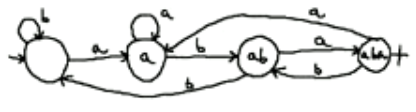
\includegraphics{t2-3.png}

\end{easylist}

\subsection{Autómatas finitos indeterministas (NFA)}
\begin{easylist}[itemize]
& Los autómatas finitos no deterministas son una extensión de los autómatas finitos deterministas. Es extraño; las ejecuciones no están unívocamente definidas. Tienen diversos caminos de ejecución que puede escoger de manera no determinista.

& Ejemplo. Tiene algo especial, el estado inicial tiene dos transiciones con $a$: una que va al propio estado y otra que va a otro estado.

\ \begin{tikzpicture}[->,>=stealth',shorten >=1pt,auto,node distance=2.8cm,semithick]

  \node[initial,state]      (A)                 {$A$};
  \node[initial,state]      (B) [right of=A]    {$B$};
  \node[initial,state]      (C) [right of=B]    {$C$};
  \node[accepting, state]   (D) [right of=C]    {$D$};

  \path (A) edge [loop above] node {$a, b$} (A)
        (A) edge              node {$a$}    (B)
        (B) edge              node {$a, b$} (C)
        (C) edge              node {$a, b$} (D);
\end{tikzpicture}

& En el último estado, no hay transiciones. Al leer un símbolo no vamos a ningún estado.
& Ejemplo de lectura de la entrada con la palabra $abbaba$. Existen diversas ejecuciones.
&& Una posible ejecución es quedarse siempre en el estado inicial. La palabra se rechazaría.
&& Otra ejecución es seguir los estados $A$, $B$, $C$ y $D$. Como no tenemos transiciones a partir del último estado, acabamos la ejecución y es una ejecución rechazadora.
&& Otra posible es hacer $abb$ en el primer estado, $a$ en el $B$, $b$ en $C$ y $a$ en $D$. En este caso sí que se aceptaría la palabra.
& Por definición, el conjunto de palabras aceptadas por el autómata es el conjunto de palabras tales que existe una ejecución aceptadora.
& En este caso, se aceptan las palabras que tienen una $a$ en la tercera posición comenzando por el final. Es decir, $[a,b]^*a[a,b]^2 = \{w \in \{a,b\}^* \colon \exists x, y \colon (w = xay \land |y| = 2)\}$.
& Es un error pensar que los autómatas finitos no deterministas tienen ``probabilidad'' de aceptar o no. Recordemos que una palabra se acepta si \textit{existe} una ejecución que llega a un estado aceptador.
& Todo autómata indeterminista se puede convertir en uno determinista que reconoce el mismo lenguaje. El autómata determinista simula todas las ejecuciones posibles del estado determinista.

& Para ello, vamos mirando cada estado adónde puede ir y lo que recuerda.
& Ejemplo (\textit{mirad el vídeo correspondiente}):
&& Indeterminista (enunciado).

\ \begin{tikzpicture}[->,>=stealth',shorten >=1pt,auto,node distance=2.8cm,semithick]

  \node[initial,state]      (A)                 {$A$};
  \node[initial,state]      (B) [right of=A]    {$B$};
  \node[initial,state]      (C) [right of=B]    {$C$};
  \node[accepting, state]   (D) [right of=C]    {$D$};

  \path (A) edge [loop above] node {$a, b$} (A)
        (A) edge              node {$a$}    (B)
        (B) edge              node {$a, b$} (C)
        (C) edge              node {$a, b$} (D);
\end{tikzpicture}

&& Determinista (resultado).

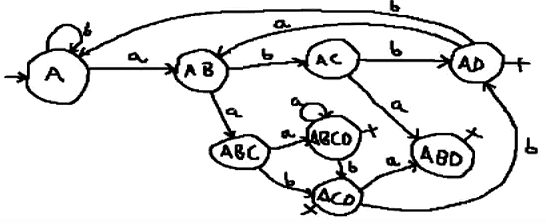
\includegraphics{t2-5.png}

\end{easylist}


\subsection{Notaciones de DFA y NFA (1)}
\subsubsection{Notaciones de DFA}
\begin{easylist}[itemize]
& Podemos usar notación por grafos.

\ \begin{tikzpicture}[->,>=stealth',shorten >=1pt,auto,node distance=2.8cm,semithick]

  \node[initial, accepting, state] (A)  {$0$};
  \node[state] (B) [right of=A] {$1$};

  \path (A) edge [loop above] node {$b$} (A)
        (B) edge [loop right] node {$b$} (B)
        (A) edge [bend left] node {$a$} (B)
        (B) edge [bend left] node {$a$} (A);
\end{tikzpicture}

& También podemos utilizar una tabla. Al principio de las filas ponemos los estados, y en el principio de las columnas ponemos los símbolos del alfabeto de entrada. Para cada casilla, indicamos el estado al que vamos a parar si, en la correspondiente fila leemos el símbolo de la correspondiente columna. Por ejemplo, si leemos una $a$ en el estado $0$, saltaremos al estado $1$. Normalmente, utilizamos $\to$ y $\dag$ para estados inicial y aceptadores, respectivamente. A veces, no se dibuja la flecha dando así a entender que el inicial es el de la primera fila.

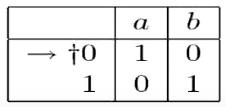
\includegraphics{t2-7.png}

& También se pueden representar por la tupla $\langle Q, \Sigma, \delta, q_0, F\rangle $.

& Podemos extender la función $\delta$ para que funcione también con palabras, no solo con símbolos del alfabeto. A esto se le llama la \textit{función de transición extendida}, y tiene la forma $\delta \colon Q \times \Sigma ^*  \to Q$.

& Intuitivamente, dado un estado y una palabra, la función de transición extendida devuelve el estado resultante de leer esta palabra a partir del estado dado.

& Por simplicidad, podemos escribir $\delta(q, a)$ por $q\cdot a$ o, simplemente, $qa$.

& Si aplicamos la palabra vacía a un estado, nos quedamos en el mismo estado: $q\lambda = q$. Es decir, $\delta(q, \lambda) = q$.

& Cualquier estado operado con una concatenación de palabras da como resultado operar primero el estado con la primera palabra y el estado resultante operarlo con la segunda palabra: $q(xy) = (qx)y$. 

& Otra propiedad: $q(a_1a_2\cdots a_n) = (\cdots ((qa_1)a_2)\cdots)a_n$.

& El lenguaje reconocido por un DFA se puede escribir como $\mathcal L (A) = \{w \colon q_0 w \in F\}$. Es decir, son todas aquellas palabras $w$ tales que, a partir del estado inicial $q_0$, llegan a un estado aceptador cualquiera (un elemento de $F$).

& También podemos definir el lenguaje reconocido por un DFA pero a partir de un estado concreto $q$ así: $\mathcal L(A, q) = \{w \colon qw \in F\}$.

& A un lenguaje se le dice \textit{regular} si y solo si existe un DFA tal que lo reconoce: $\mathcal L \in \textrm{Reg} \iff \exists A \in \textrm{DFA} \colon \mathcal L(A) = L$.
\end{easylist}

\subsubsection{Notaciones de NFA}
\begin{easylist}[itemize]
& Mismas definiciones que DFA, pero con algunos cambios. Se siguen pudiendo representar como grafos.

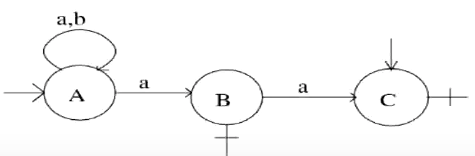
\includegraphics{t2-8.png}

& Permiten transiciones múltiplemente definidas (el estado $A$ tiene dos transiciones con la $a$), o no definidas, como pasa con la $b$ en $B$ y $C$.

& Además, admiten múltiples estados iniciales.

& Una palabra es aceptada si existe una ejecución aceptadora. Es decir, si existen un estado inicial y otro final tal que la lectura de la palabra en el estado inicial lleva al estado final.

& La representación en tabla es la misma. Puede haber más de un estado destino en cada casilla, o puede no haber ninguno.

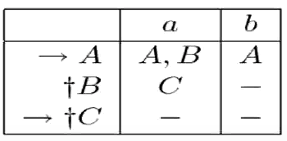
\includegraphics{t2-9.png}

\end{easylist}

\subsection{Notaciones de DFA y NFA (2)}
\subsubsection{Notaciones de NFA (continuación)}

\begin{easylist}[itemize]
& Diferencia como representación de tupla respecto los DFA: ahora no tenemos un estado inicial $q_0$, sino que podemos tener varios. Así, un NFA es una tupla $\langle Q, \Sigma, \delta, I, F\rangle$ (notad el uso de $I$ en vez de $q_0$ a diferencia de los DFA).

& Como ahora podemos ir a parar a distintos estados a partir de un estado, la función de transición también cambia su definición. Dado un estado y un símbolo, nos da como resultado un subconjunto del conjunto de estados. Es decir, $\delta \colon Q \times \Sigma \to 2^Q$.

& También notamos que $\delta \subseteq Q \times \Sigma \times Q$.

& Podemos extender la función de transición para aplicarla a un conjunto de estados y un símbolo: $\delta \colon 2^Q \times \Sigma \to 2^Q$.

& La imagen de un par (conjunto de estados, símbolo) es la unión de las imágenes de cada estado del conjunto y el símbolo. Es decir, $\delta(\{q_1, \dots, q_m\}, a) = \delta(q_1, a) \cup \dots \cup \delta(q_m, a)$. Intuitivamente, esto nos dice a qué estados podemos ir a parar si nos encontramos en algún estado de un conjunto fijado.

& Podemos extender la función de transición todavía más a conjuntos de estados y palabras cualesquiera, y no necesariamente a símbolos del alfabeto. Esto es, $\delta \colon 2^Q \times \Sigma^* \to 2^Q$. Esto se hace de manera totalmente análoga al caso de los DFA.

& La palabra vacía, $\lambda$, nos deja donde está: $\delta(\{q_1, \dots, q_m\}, \lambda) = \{q_1, \dots, q_m\}$.

& Y, al aplicar sobre la concatenación, primero se aplica sobre la primera palabra y, después, sobre la segunda: $\delta(\{q_1, \dots, q_m\}, xy) = \delta(\delta(\{q_1, \dots, q_m\}, x), y)$.

& Lenguaje aceptado por un FA: $\mathcal L(A) = \{w \colon \delta(I, w) \cap F \neq \varnothing\}$. Esto es, el conjunto de palabras para las que existe una ejecución aceptadora comenzando a partir de alguno de los estados iniciales.

& El proceso de determinización es sencillo a partir de la tabla.

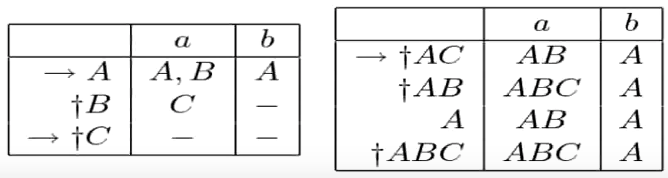
\includegraphics[width=10cm]{t2-10.png}

& Ponemos, como estados aceptadores, aquellos que incluyen en su nombre algún estado aceptador de la tabla de la izquierda.
\end{easylist}

\subsubsection{\texorpdfstring{$\lambda$}{Lambda}-NFA}
\begin{easylist}[itemize]
& Una $\lambda$-transición es una transición etiquetada con la palabra vacía.

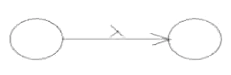
\includegraphics{t2-11.png}

& Esta transición se puede efectuar o no, de manera que los $\lambda$-NFA pueden tener varias ejecuciones diferentes para una misma palabra, como ya pasaba en los NFA en general.

& La noción de aceptación de una palabra por parte de un $\lambda$-NFA es la misma que para NFA. Es decir, decimos que el autómata acepta una palabra si existe una ejecución aceptadora para esta palabra.

& Los $\lambda$-NFA son igual de expresivos que los DFA. Es decir, tan solo pueden reconocer lenguajes regulares.

& Cualquier autómata con $\lambda$-transiciones se puede convertir en uno sin $\lambda$-transiciones que reconozca el mismo lenguaje.

& Para poder efectuar esta conversión, tenemos que añadir algunas cosas al autómata. 

& $\delta \subseteq Q \times (\Sigma \cup \{\lambda\}) \times Q$.

& Si hay algún camino con símbolos $\lambda$, podemos anticiparnos y añadir a mano otra transición, de manera que cuando borremos los $\lambda$ todavía tengamos el camino. Notamos que igual podíamos llegar de un estado a otro ejecutando las $\lambda$-transiciones.

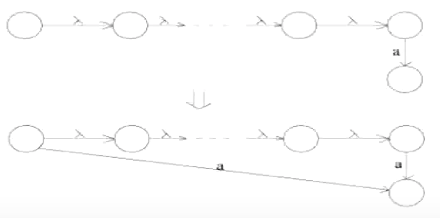
\includegraphics{t2-12.png}

& Si tenemos un camino de $\lambda$-transiciones que lleva hacia un estado aceptador, entonces ponemos el primero como aceptador, anticipándonos, de nuevo.

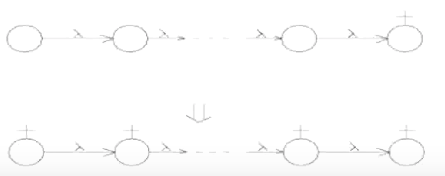
\includegraphics{t2-13.png}

& Hecho esto, ya podemos borrar las $\lambda$-transiciones del $\lambda$-NFA y obtenemos un NFA equivalente.
\end{easylist}


\subsection{Operaciones sobre Reg (1)}

Cuando operamos dos lenguajes regulares con ciertas operaciones conocidas, el resultado es otro lenguaje regular. En esta sección veremos la intersección, unión y complementario de lenguajes.

\subsubsection{Intersección y unión}
\begin{easylist}[itemize]
& Los lenguajes regulares son cerrados por intersección y unión. Esto es, que si $L_1, L_2 \in \textrm{Reg}$, entonces $L_1 \cap L2$ y $L_1 \cup L_2$ pertenecen a $\textrm{Reg}$.

& Vamos a analizar un ejemplo.

El autómata de arriba reconoce las palabras sobre $\{a,b\}$ con un número par de $a$s, y el de abajo reconoce las palabras sobre $\{a,b\}$ con un número par de $b$s.

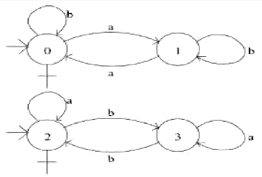
\includegraphics{t2-14.png}

& Para obtener el autómata \textit{intersección}, construiremos un autómata que simule estos dos.


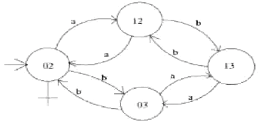
\includegraphics{t2-15.png}

& Este autómata recuerda en qué estado se encuentran los dos anteriores con una palabra leída hasta el momento.

& Por ejemplo, cuando no hemos leído nada en ningún autómata, debemos recordar que ambos autómatas se encuentran en sus estados iniciales. Por eso, recordamos los estados 0 y 2 respectivamente.

& Si leemos una $a$, en el primer autómata nos vamos al estado $1$, y en el segundo, al $2$. Por tanto, iremos al estado $12$.

& Si leemos una $a$ desde $12$, como desde $1$ pasamos a $0$, y desde $2$ seguimos quedándonos en $2$, pasamos, pues, al estado $02$. Y así sucesivamente.

& Si queremos reconocer la intersección, debemos aceptar palabras tales que, en ambos autómatas, nos lleven a estado aceptador. Por eso, ponemos como estado aceptadores aquellos que recuerden que ambos autómatas se encuentran en estado aceptador. En el caso anterior, solo $02$ es aceptador.

& Si quisiésemos reconocer la unión, la elección de los estados aceptadores es diferente. Aceptamos las palabras que aceptan alguno de los dos autómatas. Los estados aceptadores serán los que recuerden que alguno de los dos autómatas ha llegado hasta un estado aceptador. En nuestro caso, $02$, $12$ y $03$ serían aceptadores.

& Vamos a ver lo anterior, ahora, de manera formal. Supongamos que tenemos los autómatas $A_1 = \langle Q_1, \Sigma, \delta_1, q_{01}, F_1\rangle$ y $A_2 = \langle Q_2, \Sigma, \delta_2, q_{02}, F_2\rangle$.

& Definimos el autómata intersección, denotado abusivamente por $A_1 \cap A_2$, como $\langle Q_1 \times Q_2, \Sigma, \delta, \langle q_{01}, q_{02}\rangle, F_1 \times F_2\rangle$. Este autómata tiene como estados las parejas de estados de los dos autómatas anteriores, como estado inicial la pareja de estados iniciales de los dos autómatas anteriores, y como estados aceptadores, todas las parejas de estados aceptadores de los dos autómatas anteriores, y, como función de transición, $\delta(\langle q_1, q_2\rangle, a) = \langle\delta_1(q_1, a), \delta_2(q_2, a)\rangle$. Esto es, a cada par de estados de $A_1$ y $A_2$ les asigna sus estados transición correspondientes por $\delta_1$ y $\delta_2$.

& Esta descripción formal no se corresponde exactamente a la idea anterior del dibujo, porque algunas parejas de estados sean inaccesibles. En estos casos, no las consideraremos.

& Lo más recomendable para hacer la intersección de autómatas es mediante tablas.

& \textit{$\triangle$ Ejercicio: transformar a tablas los dos autómatas anteriores}.

& Definimos el autómata intersección, denotado abusivamente por $A_1 \cup A_2$ de manera parecida al autómata unión. En este caso es $\langle Q_1 \times Q_2, \Sigma, \delta, \langle q_{01}, q_{02}\rangle, (F_1 \times Q_2) \cup (Q_1 \times F_2)\rangle$. La única diferencia, como hemos visto antes, será en cuáles son los estados acepadores. En este caso, necesitamos, como estados aceptadores a una pareja tal que, o bien el primero es aceptador del primer autómata o bien el segundo es aceptador del segundo autómata.

& Estos autómatas reconocen los lenguajes intersección y unión. Esto es, $\mathcal L(A_1 \cap A_2) = \mathcal (A_1) \cap \mathcal L (A_2)$ y $\mathcal L(A_1 \cup A_2) = \mathcal (A_1) \cup \mathcal L (A_2)$.

& Los lenguajes regulares también son cerrados por la operación de complementario. Esto es, $L \in \textrm{Reg} \implies \bar L \in \mathrm{Reg}$.
\end{easylist}


\subsubsection{Complementario}
\begin{easylist}[itemize]
& Dado un autómata $A = \langle Q, \Sigma, \delta, q_0, F\rangle$, su complementario es $\bar A = \langle Q, \Sigma, \delta, q_0, Q - F\rangle$. Este autómata acepta las palabras que no acepta $A$, y viceversa. Lo único que hacemos es intercambiar estados aceptadores y rechazadores en la descripción formal del autómata.

& $\overline{\mathcal L(A)} = \mathcal L(\bar A)$.

& Esta idea no funciona con autómatas indeterministas. Esto se debe a que en autómatas indeterministas, una palabra es aceptadora si existe alguna ejecución que lleva a un estado aceptador. Pero puede pasar que una palabra llegue a estados aceptadores y rechazadores. Por esta razón, antes de aplicar la operación de complementario hay que determinizar el autómata.
\end{easylist}

\subsection{Operaciones sobre Reg (2)}
\subsubsection{Concatenación}
\begin{easylist}[itemize]
& Los lenguajes regulares son cerrados por la operación de concatenación. Es decir, $L_1, L_2 \in \text{Reg} \implies (L_1 \cdot L_2) \in \text{Reg}$. Esto es, que si existen autómatas para ambos lenguajes, entonces también existe el autómata del lenguaje de su concatenación.

& Para convencernos de ello, supongamos que el autómata de la izquierda reconoce $L_1$, y, el de la derecha, $L_2$. 

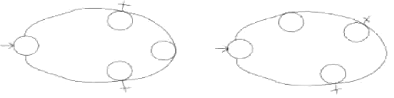
\includegraphics{t2-16.png}


& Recordemos que el lenguaje concatenación es el formado por aquellas palabras que son concatenación de palabras formadas por concatenación de una palabra de $L_1$ con una palabra de $L_2$.

& Para construir un autómata de su concatenación, hay que añadir $\lambda$-transiciones desde los estados aceptadores del primer autómata hasta el estado inicial del segundo autómata. Además, los estados aceptadores del primer autómata dejan de ser aceptadores en el nuevo autómata. Y el estado inicial del segundo autómata deja de serlo.

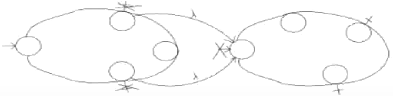
\includegraphics{t2-17.png}


& Justificación de que el autómata anterior reconoce el lenguaje concatenación. Por un lado, cualquier palabra $w$ del lenguaje concatenación se puede partir en dos partes, $w_1$ y $w_2$ de $L_1$ y $L_2$, respectivamente. Como $w_1$ es de $L_1$, esta nos lleva del estado inicial del autómata de $L_1$ a un aceptador del primer autómata. Esta ejecución se puede reproducir en el autómata concatenación, y ejecutar después la $\lambda$-transición correspondiente hacia el estado inicial del segundo autómata. Análogamente, $w_2$ nos lleva a un estado aceptador del segundo autómata. Esta ejecución se puede realizar de la misma manera en el autómata concatenación, resultando así que la composición con la anterior ejecución nos da una ejecución aceptadora de $w$. Así pues, toda palabra del lenguaje concatenación es aceptada por este nuevo autómata.

& Nos falta justificar el sentido contrario, esto es, que toda palabra aceptada por el autómata es del lenguaje concatenación. Pero esto es sencillo, pues toda ejecución aceptadora en el autómata concatenación ha de pasar en algún momento por alguna $\lambda$-transición. Por tanto, esta palabra tendrá una ejecución desde el estado inicial del primer autómata hasta un estado aceptador del primer autómata, y lo que queda de la palabra nos lleva desde el estado aceptador del segundo autómata a un estado final del segundo autómata. Esto justifica que la palabra se puede partir en una subpalabra de $L_1$ y de $L_2$. Por tanto, la palabra es del lenguaje concatenación.

\end{easylist}


\subsubsection{Estrella}
\begin{easylist}[itemize]
& Vamos a ver ahora que los lenguajes regulares son cerrados por la operación estrella. Esto es, que si existe un autómata que reconoce un lenguaje, entonces también existe otro que reconoce su estrella: $L \in \textrm{Reg} \implies L^* \in \textrm{Reg}$.

& Recordamos que la estrella de un lenguaje $L$ es el lenguaje de las palabras que se obtienen al concatenar palabras de $L$. Por tanto, queremos aceptar subpalabras que nos lleven del estado inicial a algún estado aceptador. 

& Para reconocer el lenguaje estrella, solo tenemos que añadir $\lambda$-transiciones entre todos los estados aceptadores al estado inicial.

& Además, si el estado inicial del autómata no es aceptador, hay que añadir un estado inicial adicional que sea aceptador, para aceptar también la palabra vacía.

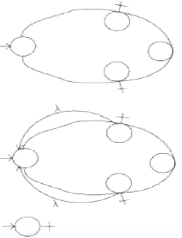
\includegraphics{t2-18.png}


& \textit{$\triangle$ Ejercicio: justificar que el autómata estrella reconoce la estrella del lenguaje original}.
\end{easylist}

\subsubsection{Reverso}
\begin{easylist}[itemize]
& Vamos a ver ahora que los lenguajes regulares son cerrados por la operación reverso. Esto es, que si existe un autómata que reconoce un lenguaje, entonces también existe otro que reconoce su reverso: $L \in \textrm{Reg} \implies L^R \in \textrm{Reg}$.

& Sea el primer autómata uno que reconozca $L$. Las palabras de $L$ son las que nos llevan del estado inicial a algún estado aceptador. Por tanto, una palabra de $L^R$ nos llevaría de un estado aceptador al estado inicial siguiendo las flechas en sentido inverso. 

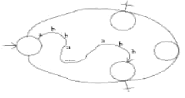
\includegraphics{t2-19.png}


& Basándonos esta idea, definimos el estado reverso de esta manera. Si $A = \langle Q, \Sigma, \delta, q_0, F\rangle$, entonces $A^R = \langle Q, \Sigma, \{qa \to q'|(q'a\to q) \in \delta\}, F, \{q_0\}\rangle$. El autómata reverso tiene los mismos estados y el mismo alfabeto que el original; sus transiciones son las del original pero giradas. Es decir, si en el original íbamos de $q'$ a $q$ después de leer una palabra $a$, en el reverso vamos de $q$ a $q'$ después de leer la palabra $a$. Además, se intercambian estados iniciales y aceptadores. El conjunto de estados aceptadores contiene ahora, únicamente, el estado inicial del autómata original.

& \textit{$\triangle$ Ejercicio: justificar que $\mathcal L(A^R) = (\mathcal L(A))^R$.}
\end{easylist}


\subsubsection{Técnica de obtención de DFA o NFA por descomposición}
\begin{easylist}[itemize]
& Vamos a ver una técnica que permite construir un autómata que reconoce lenguajes complejos. Para eso nos basaremos en las operaciones de clausura que hemos visto anteriormente.

& La idea consiste en formalizar el lenguaje, y después ir descomponiendo esta formalización mediante operaciones intermedias hasta que el lenguaje de partida sea descrito en función de lenguajes sencillos para los cuales sea fácil obtener un autómata autómaticamente. No es una técnica infalible.

& Ejemplo. Queremos obtener el autómata que reconozca el lenguaje de las palabras sobre $a$ y $b$ tales que, a la derecha de toda $a$ queda una palabra con un número par de $b$s. Esto es, el lenguaje $L = \{w \in \{a,b\}^* \colon \forall x,y \colon (w = xay \implies |y|_b \in \dot 2\}$.

& Encontrar un autómata directamente es difícil. La formalización anterior incluye un cuantificador universal. Habitualmente, es más sencillo encontrar autómatas para propiedades existencialmente cuantificadas. Por este motivo, calcularemos el lenguaje complementario a $L$, formalizable por $\bar L = \{w \in \{a,b\}^* \colon \exists x, y \colon (w = xay \land |y|_b \notin \dot 2\}$.\footnote{Se ha aplicado que $\neg \forall x (p(x)) \equiv \exists x (\neg p(x))$ y la definición de implicación: $p \to q \equiv \neg p \lor q$.} Como los lenguajes son cerrados por complementario, si encontramos un autómata para $\bar L$, podremos convertirlo en uno para $L$. 

& Nótese que el existencial liga bien con la noción de aceptación en autómatas no deterministas, pues nos preguntamos por la existencia de una ejecución hacia un estado aceptador. Sería suficiente pues, con un autómata indeterminista que, de manera no determinista escoja una $a$, y después compruebe que lo que queda es un número impar de $b$.

& De todas maneras, todavía se puede descomponer más el autómata. $\bar L = \{a,b\}^* \{a\} \{y \in \{a,b\}^* \colon |y|_b \notin \dot 2\}$. En definitiva, tenemos que $w$ se parte en tres subpalabras. La primera subpalabra es una cualesquiera, la segunda es una $a$ y la tercera tiene un número impar de $b$s. Así pues, $\bar L$ es la concatenación de estos tres lenguajes. Ahora sí que podemos obtener autómatas sencillos.

& \textit{$\triangle$ Ejercicio: dibujar el autómata para $L$ a partir de la descomposición anterior}.


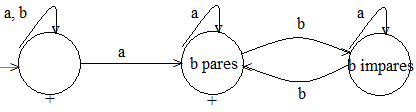
\includegraphics{t2-20.png}

& Observación: también podríamos haber calculado el reverso fácilmente, como $L^R = \{w \in \{a,b\}^* \colon \forall x, y \colon (w = xay \implies |x|_b \in \dot 2\}$. Esto es, las palabras que tienen un número impar de $b$s seguidas de $a$ y de una palabra cualquiera.

\end{easylist}


\subsection{Operaciones sobre Reg (3)}


\subsubsection{Morfismo directo}
\begin{easylist}[itemize]
& Si hay un autómata que reconoce un lenguaje, entonces también hay otro que reconoce la imagen de este lenguaje por un morfismo: $L \in \textrm{Reg} \land \sigma(xy) = \sigma(x)\sigma(y) \implies \sigma(L) \in \textrm{Reg}$.

& La construcción la haremos mediante un ejemplo. Suponemos que tenemos el morfismo $\sigma \colon \{a,b,c\}^* \to \{0, 1\}^*$ tal que $\sigma(a) = 01$, $\sigma(b) = 1$ y $\sigma(c) = \lambda$ y el autómata de arriba de la figura para $L$. El autómata que reconoce $\sigma(L)$ es el de abajo.

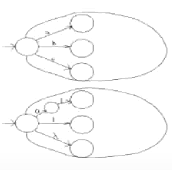
\includegraphics{t2-21.png}

& En el nuevo autómata:
&& Si tenemos una transición de tamaño uno, simplemente renombramos las etiquetas.
&& Si tenemos una transición con imagen de mayor tamaño, entonces añadimos suficientes estados intermedios nuevos.
&& Por último, si la imagen de la transición tiene tamaño cero (situación en la que la imagen es $\lambda$), entonces transformamos la transición en una $\lambda$-transición.

& Aplicamos estos cambios a todas las transiciones del autómata original.

& \textit{$\triangle$ Ejercicio: justificar que este nuevo autómata realmente reconoce el morfismo del lenguaje original.}
\end{easylist}

\subsubsection{Morfismo inverso}
\begin{easylist}[itemize]
& Los lenguajes regulares también son cerrados por morfismo inverso. Es decir, si existe un autómata que reconoce un lenguaje, entonces también hay otro que reconoce el conjunto imagen de este por un morfismo. Es decir, $L \in \mathrm{Reg} \land \sigma \colon \Sigma_1^* \to \Sigma_2^* \land \sigma(xy) = \sigma(x)\sigma(y) \implies \sigma^{-1} (L) \in \mathrm{Reg}$.

& Recordemos que la antiimagen de un conjunto $L$ es el conjunto de elementos cuya imagen está en $L$.

& A partir de un autómata $A = \langle Q, \Sigma_2, \delta, q_0, F\rangle$ que reconoce $L$, veamos cómo construir un autómata que reconozca $\sigma^{-1}(L)$.

& El autómata antiimagen tiene los mismos estados que $A$, pero su alfabeto es el correspondiente al dominio de $\Sigma_1$. Tendrá los mismos estados aceptadores y estado inicial que $A$, y la principal diferencia está en las reglas. $\sigma^{-1}(A) = \langle Q, \Sigma_1, \delta', q_0, F\rangle$.\footnote{En el minuto 2:15 del vídeo hay un error en esta definición. Aquí está correctamente escrita.}

& Hay que definir $\delta'$ para parejas (estado de $Q$, símbolo de $\Sigma_1$), obteniendo como resultado otro estado de $Q$: $\delta' \colon Q \times \Sigma_1 \to Q$.

& El estado al que iremos a parar desde $q$ después de leer $a$ lo definimos como el estado al que íbamos a parar en el autómata original después de leer la imagen original desde $q$. Esto es, $\delta'(q,a) = \delta(q, \sigma(a))$. Nótese que la imagen de $a$, $\sigma(a)$ no necesariamente tiene tamaño 1. No obstante, esto no es un problema, porque podíamos extender la definición de $\delta$ para pares (estado, palabra).

& Formalmente, $\sigma^{-1}(L) = \sigma^{-1}(\mathcal L(A)) = \mathcal L (\sigma^{-1}(A))$.\footnote{Consultad \url{http://youtu.be/L8HtVewJfzM} a partir del minuto 3:23 para la demostración (totalmente formal y nada intuitiva) de esta propiedad.}
\end{easylist}


\subsection{Minimización de DFA (1)}
\begin{easylist}[itemize]
& En esta sección y en las siguientes veremos que, en todos los DFA que reconocen un lenguaje fijado, hay uno concreto que tienen menos estados estados que cualquiera de los otros, y que llamaremos \textit{DFA mínimo}.

& Empezamos analizando este ejemplo de DFA.

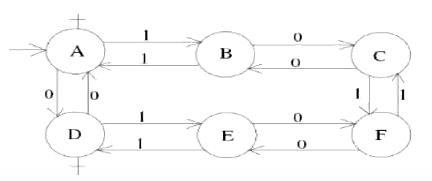
\includegraphics{t2-22.png}

& Imaginemos que estamos en medio de una ejecución y que nos encontramos, o bien en el estado $A$, o bien en el $D$, pero no sabemos en cuál de los dos. Si de repente la ejecución acaba, en ambos casos aceptaremos. En caso contrario, si leemos un $0$, seguimos en $A$ o $D$, sin saber en cuál. Si leemos un $1$, pasaremos al estado $B$ o $E$; no sabemos cuál. Si la ejecución acaba, sea cual sea el caso, acabamos. En cambio, si leemos un $0$, iremos a $C$ o $F$, sin saber en cuál. Si acaba la ejecución, rechazamos. En caso contrario, si ahora leemos un $1$, iremos a $C$ o $F$ sin saber a cuál, etc.

& Todo este discurso nos puede servir para intuir que los estados $A$ y $D$ son equivalentes en el sentido de que las palabras aceptadas empezando desde $A$ son las mismas que aquellas aceptadas empezando desde $D$. Los estados $B$ y $E$, y $C$ y $F$ son también equivalentes en este sentido.

& Esta noción de equivalencia nos servirá para reducir el tamaño del DFA. Por ejemplo, intuitivamente, parece que la transición de $E$ a $D$ con un $1$ la podríamos desviar hacia $A$, ya que desde $A$ se reconoce el mismo lenguaje desde $D$. Y la transición de $A$ a $D$ la podríamos redirigir también hacia $A$ (un bucle). Así $D$ ya no sería accesible y lo podríamos borrar.

& Vamos a concretar estas ideas con el objetivo de reducir el tamaño de un DFA hasta encontrar el DFA mínimo reconociendo el mismo lenguaje.

& Definimos la siguiente relación entre estados de $A = \langle Q, \Sigma, \delta, q_0, F \rangle$ que denotamos por $q\sim_A q'$ o como $q \sim q'$ así: dos estados $q$ y $q'$ son equivalentes o indistinguibles ($q \sim q'$) si los lenguajes reconocidos desde ellos son equivalentes: $\mathcal L (A, q) = \mathcal L (A, q')$. Esto es, que para toda palabra $w$, desde $q$ llegamos a estado aceptador después de leer $w$ si y solo si desde $q'$ llegamos a estado aceptador después de leer $w$: $\forall w \in \Sigma^* \colon (qw \in F \iff q'w \in F )$.

& No es difícil comprobar que la relación anterior es de equivalencia: es reflexiva, simétrica y transitiva.

& Recordamos que, siempre que tenemos una relación de equivalencia sobre un conjunto, se puede hablar del conjunto cociente, $Q / \sim$, que es la partición en clases de equivalencia. En nuestro ejemplo anterior,  el conjunto cociente es $Q/ \sim = \{\{A, D\},\{B, E\}, \{C, F\}\}$.

& La clase de equivalencia de un elemento $q$ es $[q]$. Así, $[A] = [D] = \{A, D\}$ en el ejemplo anterior.

& Vamos a demostrar que, cuando dos estados son indistinguibles o equivalentes, después de leer el mísmo símbolos desde ellos, vamos a parar a una pareja de estados que también son equivalentes. Esto es que si $q \sim q'$ (también se puede escribir como $[q] = [q']$, entonces, $\forall a \in \Sigma$, $qa \sim q'a$; o lo que es lo mismo, que $[qa] = [q'a]$.\footnote{Hay un error en el minuto 3:34 del vídeo \url{https://youtu.be/QN7V3fVZRNI} sin notificar. Las clases de equivalencia resultantes de $q$ y $q'$ son iguales, pero no están relacionadas por $\sim$.}

& Demostramos esta propiedad:
&& Comenzamos con la hipótesis de que $q$ y $q'$ son equivalentes ($q \sim q'$) y sea $a$ un símbolo cualquiera de $\Sigma$.
&& Por definición de equivalencia, tenemos que $\forall w \colon (qw \in F \iff q'w \in F)$.
&& En particular, cualquier palabra que empiece por $a$ también lo verificará: $\forall w \colon (q(aw) \in F \iff q'(aw) \in F)$.
&& Esto implica que cualquier palabra nos lleva a estao aceptador desde el estado $qa$ si y solo si nos lleva a estado aceptador desde el estado $q'a$: $\forall w\colon ((qa)w \in F \iff (q'a)w \in F)$.
&& Pero esto es precisamente $qa \sim q'a$, como queríamos demostrar.

& Dicho de otra manera, $\forall w \in \Sigma^* \colon ([q] = [q'] \implies [qw] = [q'w])$.

& El autómata cociente se deduce de las propiedades anteriores: $A/\sim = \langle Q/\sim, \Sigma, \{[q]a \to [qa]\colon q \in Q, a \in \Sigma\}, [q_0], \{[q] \colon q \in F\}\rangle$. Esto es, los estados son las clases de equivalencia, el alfabeto es el mismo, el estado inicial es la clase del estado inicial y los estados aceptadores son las clases de aquellos estados que eran aceptadores. La función de transición se define como aparece en esta definición.

& Este autómata reconoce el mismo lenguaje que el autómata original: $\mathcal L(A) = \mathcal L (A/\sim)$. Vamos a demostrarlo:

&& Esto es equivalente a decir que para toda palabra $w = a1\dots a_n$ de $\Sigma^*$, $q_0w \in F$ si y solo si $[q_0]w \in \{[q] \colon q \in F\}$, o, dicho de otra manera, que la palabra es aceptada en $A$ si y solo si es aceptada en $A / \sim$.

&& Aplicando la definición de función de transición en $A / \sim$, podemos deducir que el estado al que se va a parar después de leer $w$ desde la clase del estado inicial del autómata cociente; esto es, $[q_0]$, es la clase del estado $q_0 w$, $[q_0w]$. En definitiva: $[q_0]w = [q_0 w]$. La demostración va como sigue:

$[q_0]w = [q_0](a_1 \dots a_n) = ([q_0]a_1)(a_2 \dots a_n) = [q_0 a_1](a_2 \dots a_n) =$

$= ([q_0 a_1]a_2) (a_3 \dots a_n) = [q_0 a_1 a_2](a_3 \dots a_n) = \dots = [q_0 w]$.

&& Por tanto, hay que demostrar que $q_0 w \in F \iff [q_0w] \in \{[q] \colon q\in F\}$; pero esto es obvio, ya que, por la definición del autómata cociente, la clase de un estado es aceptadora si este estado es aceptador. Esto acaba con la demostración.

& Volviendo con el ejemplo anterior, este es el autómata cociente equivalente.

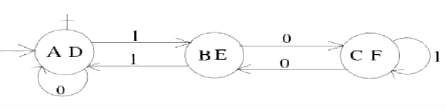
\includegraphics{t2-23.png}

\end{easylist}




\subsection{Minimización de DFA (2)}
\begin{easylist}[itemize]
& En esta sección veremos cómo calcular la partición en clases de estados indistinguibles de un DFA.

& Sea $A = \langle Q, \Sigma, \delta, q_0, F\rangle$. Recordamos que dos estados son indistinguibles cuando los respectivos lenguajes reconocidos desde $q$ y $q'$ coinciden, o, alternativamente, que cualquier palabra nos lleva a estado aceptador desde $q$ si y solo si lo hace desde $q'$. Más formalmente: $q \sim_A q' \equiv q \sim q' \equiv \mathcal L(A,q) = \mathcal L(A, q') \equiv \forall w \in \Sigma^* \colon (qw \in F \iff q'w \in F)$.


& Para ver qué parejas de estados son equivalentes, comprobamos esta propiedad. Empezaremos con palabras de longitud 0, después, de longitud 1, y así sucesivamente.

& Con esta finalidad nos será útil construir una relación de equivalencia para cada longitud.

& Con $q\sim_{A, k} q'$ (o simplemente $q \sim_k q'$ si se sobreentiende el autómata $A$) notamos que $q$ y $q'$ son dos estados $k$-indistinguibles. Por definición, dos estados son $k$-indistinguibles si $\mathcal L(A, q) \cap \{w \in |w| \leq k\} = \mathcal L(A, q') \cap \{w \in |w| \leq k\}$. Esto es, si los lenguajes reconocidos por ambos coinciden considerando solo las palabras de longitud hasta longitud $k$. Equivalentemente, también $q \sim q'$ si $\forall w \in \Sigma^*$ tenemos que $|w| \leq k \implies (qw \in F \iff q'w \in F)$.

& La $k$-indistinguibilidad es una relación de equivalencia.

& Tampoco es difícil convencerse que dos estados son indistinguibles si son $k$-indistinguibles para todo natural $k$: $q \sim q' \iff \forall k \geq 0 \colon q \sim_k q'$.

& La $k$-indistinguibilidad se puede definir también recursivamente. Si $k = 0$ (la palabra a leer será $\lambda$, y, por tanto, no nos movemos del estado) entonces $q\sim_0 q' \equiv (q \in F \iff q' \in F)$ es decir: o bien los dos son aceptadores o bien los dos son rechazadores.

& Para $k \geq 1$, $q \sim_k q'$ es equivalente a $q\sim_{k-1} q'$ y $\forall a \in \Sigma \colon (qa \sim_{k-1} q'a)$. Esto es, que dos estados $q$ y $q'$ son $k$-indistinguibles si son $k-1$ indistinguibles y, para todo símbolo $a$, la pareja de estados a la que vamos a parar leyendo $a$ también tiene que ser $k-1$-indistinguibles; pues si se pudieran distinguir con una palabra de longitud $k-1$, entonces $q$ y $q'$ se podrían distinguir con una palabra de longitud $k$.

& Podemos utilizar la definición recursiva anterior para calcular $Q/\sim$ o, abusivamente, $\sim$, en el autómata ya visto que tenéis a continuación.

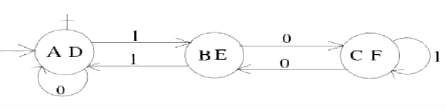
\includegraphics{t2-23.png}

& La partición en 0-indistinguibles es la partición en, por un lado los estados aceptadores y, en por el otro, los rechazadores.

$\sim_0 \colon \{A,D\} \{B, C, E, F\}$.

& Ahora, miramos dos a dos en cada conjunto para ver si vamos a parar a estados de la misma clase. Si lo hacen, no tocamos las particiones. Sino, agregamos particiones.

& La partición $\{A, D\}$ no la podemos separar, porque:
&& Si leemos un $0$, desde $A$ llegamos a $[A]$, y desde $D$ también.
&& Si leemos un $1$, desde $A$ llegamos a $[B]$, y desde $D$ también (recordad que $[B] = \{B, C, E, F\}$.

& En cambio, si comparamos $B$ y $C$, si leemos un $0$ nos quedamo en $[B]$, pero si leemos un $1$, en $B$ vamos a $[A]$ y en $C$ nos quedamos en la misma clase $[F]$. Por tanto, los separamos.

& Con $C$ y $E$ por ejemplo, si leemos un $0$ vamos a parar a $[B]$ y a $[F]$, que ya hemos visto que pertenecen a clases diferentes.

En definitiva, $\sim_1 : \{A, D\}\{B, E\}\{C, F\}$.

& Para $\sim_2$ ya no podemos refinar más las particiones (porque ya no podemos reducir más las particiones).

& Por tanto, $\sim_k \colon \{A, D\}\{B, E\}\{C, F\}$, para toda $k \geq 1$.

& Cuando $\sim_k = \sim_{k+1}$, ya no cambia más.

& No se puede refinar un DFA más del número de estados que contiene.

& En definitiva, $\sim \colon \{A, D\}\{B, E\}\{C, F\}$, también llamado \textit{conjunto cociente}.

\end{easylist}

\subsection{Minimización de DFA (3)}
En esta sección se explica por qué el método empleado en la sección anterior para generar DFA mínimos realmente genera DFA mínimos. Esto es, que dados dos autómatas minimizados $A_1$ y $A_2$ que describen el mismo lenguaje, entonces forzosamente $A_1$ y $A_2$ son iguales excepto por renombramiento de los estados por una biyección total $f$.

No resulta de utilidad transcribir toda la demostración; consultad el vídeo correspondiente, que es \url{https://youtu.be/ON1DM6EBX6Y}.